\section{Implementace prototypu aplikace}
V předchozí kapitole je představena architektura systému, který umožňuje běh aplikací napříč více Kubernetes clustery. V této kapitole je představen prototyp aplikace, která tuto architekturu implementuje. Pro pojmenování jednotlivých částí aplikace jsou použity pojmy definované v architektuře aplikace. Pro vytvoření aplikace byl použit programovací jazyk Golang, zkráceně Go. Go programovací jazyk byl vytvořen zaměstnanci společnosti Google v roce 2009. Go je kompilovaný staticky typovaný jazyk, který umožňuje překlad zdrojových kódů do strojového kódu. Go se snaží být jednoduchý a dobře čitelný programovací jazyk. Go obsahuje na paměť nenáročná vlákna, nazývaná goroutines, které umožňují bez větších problémů v aplikacích spustit stovky až tisíce takovýchto goroutines. Pro komunikaci mezi jednotlivými goroutinami poskytuje jazyk Go tkz. Channely. Dalším plusem jazyka Go je rychlá kompilace, stejně jako běh samotné aplikace. Go obsahuje silnou typovou kontrolu a automatickou správu paměti. Součástí specifikace jazyka Go je i jednotný formát kódu. Pro formátování nabízí jazyk nástroj gofmt. Jazyk plně podporuje UTF-8 kódování a je plně open source \cite{miek}. V jazyce Go je vytvořeno mnoho projektů například Docker nebo Kubernetes. I tento fakt je jedním z důvodů proč byl vybrán právě jazyk Golang. Kubernetes nabízí pro jazyk Go klientské knihovny, které dávají vývojářům možnost jak pracovat s Kubernetes API.\par
    Na obrázku \ref{fig:vk8s} je zobrazena komunikace jednotlivých částí aplikace. Customer \linebreak manager sleduje Customer API, složené z k8s API a Etcd databáze, ke kterému přistupují jednotliví uživatelé a vytvářejí v něm zdroje. Pokud Customer manager zjistí vytvoření nového zdroje, vytvoří událost, která tuto akci reprezentuje. Tato akce je zaslána \linebreak Minikube manageru s využitím channelu. Minikube manager obdrží tuto událost a provede stejnou akci v Minikube clusteru. Příkladem takovéto akce může být vytvoření Podu s jedním kontejnerem uvnitř. Uživatel vytvoří definici Podu v Customer API. Customer manager zjistí tuto událost a zašle definici Minikube manageru. Minikube manager přijme z channelu akci a vytvoří tuto definici v k8s clusteru. V tomto clusteru je podle definice spuštěn Pod. Minikube manager sleduje Minikube cluster a odesílá informace. Například Minikube manager odesílá přes channel 1 Customer manageru informace o stavu vytvořeného Podu, který aplikuje tyto informace do Customer API. Uživatel tak vidí informace o podu v Customer API stejně jako by se připojoval přímo do Minikube clusteru.\par


\begin{figure}[H]
  \begin{centering}
    
	  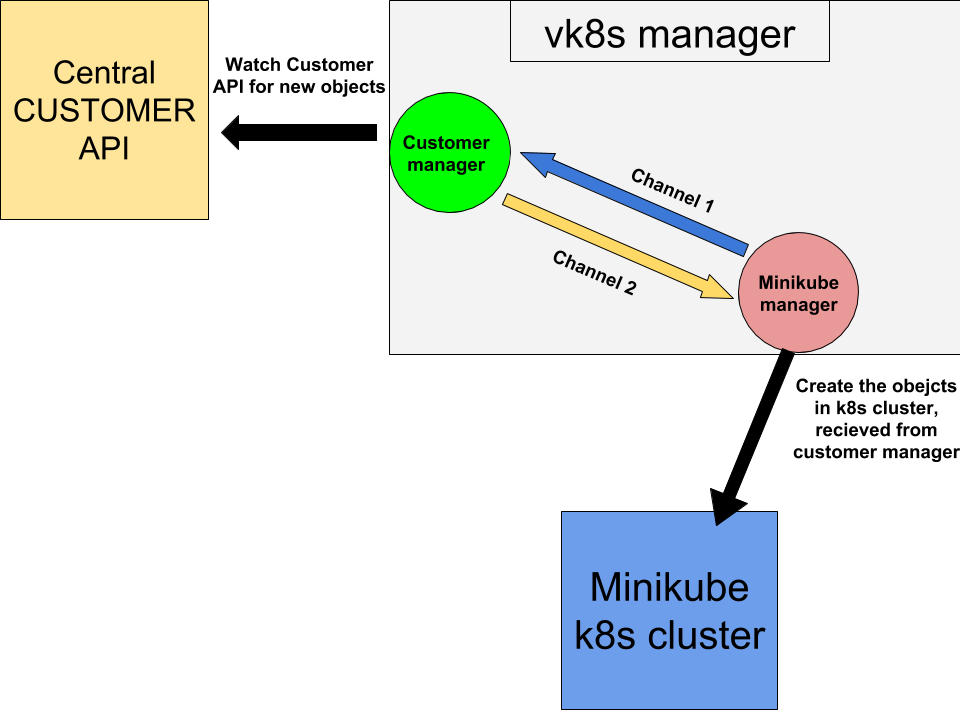
\includegraphics[width=0.8\textwidth]{images/vk8s.png}
    \par
	  \caption{Schéma vk8s manageru\label{fig:vk8s}, zdroj: vlastní tvorba}
    \end{centering}
\end{figure}

Zdrojový kód aplikace je dostupný v GitHub repozitáři\footnote[1]{\url{https://github.com/casek14/vk8s-manager}}. Struktura aplikace je uvedena v příloze \hyperref[app:struktura]{D}. Funkcionalita aplikace je rozdělena do jednotlivých balíčků (packages). Soubor main.go obsahuje instrukce jak se má aplikace spustit. Jako první je vytvořen objekt Manager, který se skládá ze dvou dalších částí. Manager je součástí balíku cluster. Jedna část, nazývaná Customer manager slouží pro interakci s centrálním k8s API. Druhou částí je Minikube manager, který interaguje s k8s clusterem. Funkce implementující vytvoření nového Managera je zobrazena na ukázce kódu \ref{lst:cluster}. Nejdříve jsou definovány jména namespaců, které budou dále využity. Poté jsou \linebreak vytvořeny dva managery, Customer Manager a Minikube Manager. Pokud vytvoření proběhlo úspěšně, metoda vrátí strukturu Manager. 

\begin{lstlisting}[caption={funkce vytvoření nového managera},label=lst:cluster]
func New() *Manager {
	log.Println("Preparing new Manager")
	customerNamespace := "mynamespace"
	customerName := "customer1"
	minikubeNamespace := fmt.Sprintf("%s-%s", customerNamespace, customerName)
	m, err := vk8s.New(&manager.Config{KubeConfigPath: minikubeKubeconfig, Namespace: minikubeNamespace, Mode: manager.Minikube})
	if err != nil {
		log.Fatalf("Unable to setup new manager, %s", err)
	}
	c, err := vk8s.New(&manager.Config{KubeConfigPath: customerKubeconfig, Namespace: customerNamespace, Mode: manager.Customer})
	if err != nil {
		log.Fatalf("Unable to setup new manager, %s", err)
	}
	return &Manager{m, c}
}
\end{lstlisting}
\par
											Implementace výše zmíněných Managerů se nachází v balíčku vk8s. Funkce \linebreak vk8s.New() v ukázce kódu \ref{lst:new} přijímá jako vstupní parametr strukturu Config z balíčku manager. Tato Config struktura obsahuje informaci o cestě k souboru kubeconfig, název namespacu a hodnotu Mode. Kubeconfig soubor se používá pro připojení a komunikaci s k8s API, obsahuje například ip adresu pro připojení k serveru nebo certifikáty k autorizaci. Hodnota Mode určuje zda bude vytvořen manager pro centrální customer API nebo pro k8s cluster minikube.\par 
\begin{lstlisting}[caption={vk8s.New() funkce pro vytvoření customer a minikube managera},label=lst:new]
func New(cfg *manager.Config) (manager.Interface, error) {
  if cfg.Mode == "" || cfg.Namespace == "" || cfg.KubeConfigPath == "" {
    return nil, fmt.Errorf("could not create new manager, incomplete configuration")
  }
  log.Printf("Preparing new %s manager", cfg.Mode)
  rc, err := k8s.NewRestConfig(k8s.Config{ConfigType: k8s.OutCluster, KubeConfigPath: cfg.KubeConfigPath})
  if err != nil {
    return nil, fmt.Errorf("Could not initialize rest config, err: %s", err)
  }
  clientset, err := kubernetes.NewForConfig(rc)
  if err != nil {
    return nil, fmt.Errorf("Could not initialize clientset, err: %s", err)
  }
  inf := informer.New(string(cfg.Mode))
  switch cfg.Mode {
    case manager.Customer:
      return &customer{vk8s{clientset, worker.New(clientset, inf), k8s.NewNamespaceObjectFromObject(clientset, &v1.Namespace{ObjectMeta: metav1.ObjectMeta{Name: cfg.Namespace}}), inf}}, nil
    case manager.Minikube:
      return &minikube{vk8s{clientset, worker.New(clientset, inf), k8s.NewNamespaceObjectFromObject(clientset, &v1.Namespace{ObjectMeta: metav1.ObjectMeta{Name: cfg.Namespace}}), inf}}, nil
    default:
      return nil, fmt.Errorf("unknown manager mode")
  }
}
\end{lstlisting}

Zmíněné managery implementují rozhraní manager.Interface, které obsahuje jednu metodu Start(inEvent, outEvent), která přijímá dva channely jako vstupní parametry. Na ukázce kódu \ref{lst:customer} je zobrazena metoda Start() pro Customer manager. Na začátku běhu funkce je ověřeno, že existuje potřebný namespace v customer API. Pokud neexistuje tak je vytvořen. V dalším kroku je vytvořen servisní účet, který bude aplikace používat pro práci s k8s API. Po vytvoření servisního účtu je spuštěna metoda Watch(outEvent), která sleduje zdroje v centrálním customer API a je detailně popsána dále v textu. Posledním krokem funkce Start() je sledování akcí na vstupním channelu. Slovo go před definicí funkce značí, že funkce bude spuštěna v goroutině, neboli \linebreak na paměť nenáročném vlákně. Uvnitř goroutiny se v nekonečném cyklu čeká \linebreak na události, které jsou obdrženy z inEvent channelu. Channely v jazyce Go fungují pro komunikaci mezi goroutinami. V tomto případě jedna goroutina do channelu zapisuje data a druhá z tohoto channelu data čte. Pokud na channelu přijde nějaká událost, je tato událost předána do volání funkce Run(), která tuto událost aplikuje do customer API. Například vytvoření nového zdroje je reprezentováno jako struktura Event s typem události Create a objekt, který má být vytvořen. Do inEvent channelu zapisuje data minikube manager, který sleduje k8s cluster, díky tomu se informace z k8s clusteru dostanou do centrálního customer API.


\begin{lstlisting}[caption={funkce Start Customer managera},label=lst:customer]
func (c *customer) Start(inEvent <-chan watch.Event, outEvent ...chan<- watch.Event) error {
	err := c.namespace.Apply()
	if err != nil {
		return fmt.Errorf("unable to start Customer k8s manager, %s", err)
	}
	log.Println("Customer k8s manager started")
	svc := &v1.ServiceAccount{ObjectMeta: metav1.ObjectMeta{Name: "default"}}
	c.CoreV1().ServiceAccounts(c.namespace.GetName()).Create(svc)
	err = c.Watch(outEvent)
	if err != nil {
		return fmt.Errorf("unable to start Customer k8s manager, %s", err)
	}
	go func() {
	log.Println("Customer watch incoming events from hyperkube")
	for {
	select {
		case ev := <-inEvent:
		// apply event int vk8s
		c.w.Run(manager.Event{ev, manager.Customer}, worker.SetNamespace(c.namespace.GetName()))
	}
	}
	}()
	return nil
}
\end{lstlisting}
\par																																					    V rámci volání funkce Start() pro customer managera je spuštěna v goroutině funkce watch, která je zobrazena v ukázce kódu \ref{lst:watch}. Úkolem této funkce je sledovat zdroje customer API. Pokud jsou například přidány nové zdroje nebo dojde k modifikaci stávajících zdrojů, Watch funkce tuto událost zaznamená a odešle informaci do minikube clusterů. Na začátku funkce jsou vytvořeny watchery zdrojů v customer API. Watcher má za úkol sledovat jeden specifický zdroj v k8s API. Jestliže dojde k přidání, \linebreak modifikaci nebo smazání zdroje je vygenerována událost, která je odeslána do channelu. Příkladem může být objekt deploymentWatcher, který sleduje zdroj Deployment \linebreak v určitém namespacu. Po vytvoření watcherů následuje spuštění goroutiny, uvnitř které se v cyklu čeká na události zaslané od jednotlivých watcherů. Pokud je na channelu, který reprezentuje události spojené s deploymentem, obdržena událost je dále odeslána do všech outEvent channelů. Tímto mechanismem obdrží k8s clustery informaci o novém deploymentu. Události z centrálního API jsou takto pomocí Manageru přeneseny do k8s clusterů. Minikube clustery obdrží na vstupním channelu informaci, kterou využijí a spustí v nich definovaný workload. Minikube manager funguje na stejném principu, s tím rozdílem, že sleduje k8s cluster a události z tohoto clusteru zasílá do customer manageru pomocí channelu, který tyto informace vkládá do centrálního customer API. 
\begin{lstlisting}[caption={funkce Watch, která sleduje Customer API zdroje},label=lst:watch]
func (c *customer) Watch(outEvent []chan<- watch.Event) error {
  log.Println("Watch for Customer cluster initiated")
  deploymentWatcher, err := c.Clientset.ExtensionsV1beta1()
    .Deployments(c.namespace.GetName()).Watch(metav1.ListOptions{})
  if err != nil {
    return fmt.Errorf("unable to establish watch for Customer k8s, %s", err)
  }
  serviceWatcher, err := c.Clientset.CoreV1().
    Services(c.namespace.GetName()).Watch(metav1.ListOptions{})
  if err != nil {
    return fmt.Errorf("unable to establish watch for Customer k8s, %s", err)
  }
  configMapWatcher, err := c.Clientset.CoreV1().
    ConfigMaps(c.namespace.GetName()).Watch(metav1.ListOptions{})
  if err != nil {
    return fmt.Errorf("unable to establish watch for Customer k8s, %s", err)
  }
  statefulSetWatcher, err := c.Clientset.AppsV1beta2().
    StatefulSets(c.namespace.GetName()).Watch(metav1.ListOptions{})
  if err != nil {
    return fmt.Errorf("unable to establish watch for Minikube k8s, %s", err)    }
  go func() {
    for {
      select {
      case ev := <-deploymentWatcher.ResultChan():
      // send deployment event into Minikube cluster
      for _, ch := range outEvent {
        ch <- ev
      }
      case ev := <-serviceWatcher.ResultChan():
      // send service event into Minikube cluster
      for _, ch := range outEvent {
        ch <- ev
      }
      case ev := <-configMapWatcher.ResultChan():
      // send config map event into Minikube cluster
      for _, ch := range outEvent {
        ch <- ev
      }
      case ev := <-statefulSetWatcher.ResultChan():
      // send statefull set event into Minikube cluster
      for _, ch := range outEvent {
        ch <- ev
      }
      }
    }
  }()
  return nil
}
\end{lstlisting}
